The first thing we need to understand is what the \gls{RF} spectrum looks like. There are plenty of electromagnetic waves around, which you may or may not be aware of. Let's quickly revise what a wave looks like, by looking at \cref{wave}\footnote{\url{https://www.bbc.com/bitesize/guides/zgf97p3/revision/1}}.

\centrefigurestart
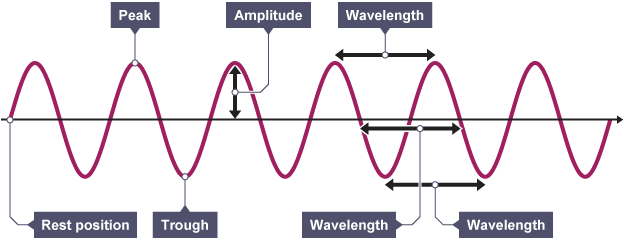
\includegraphics[width=\imgwidth]{bitesize_Wave.png}
\caption{The RF spectrum}
\label{wave}
\centrefigureend

The key thing we care about from this diagram is the wavelength because that determines how long it takes for the wave to happen; it's period. This can be used to calculate how many times it' repeats in a second, this is measured in \textit{Hertz} and is a result of the equation shown in \cref{equ:freq}. 

\begin{equation}
\text{Frequency (Hz)} = \frac{1}{\text{Time for one cycle of the wave (s)}}
\label{equ:freq}
\end{equation}

For example a signal that repeats every 2.309469 nanoseconds has a frequency of 434MHz - it repeats 434 million times a second. There are loads of different frequencies in the \gls{RF} spectrum and 434MHz fits in the \gls{uhf} part of this, as shown in \cref{spectrum}\footnote{\url{https://www.ecnmag.com/blog/2017/06/understanding-rf-spectrum}}.

\centrefigurestart
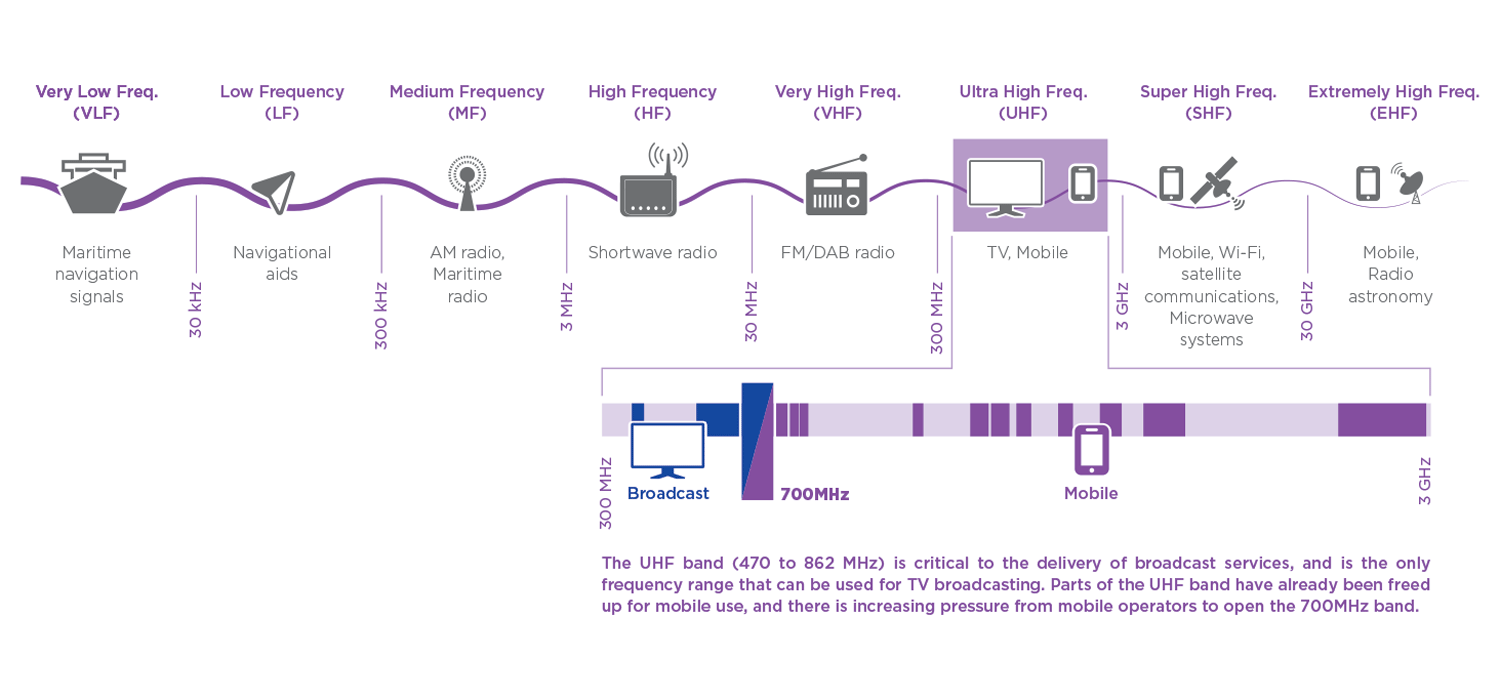
\includegraphics[width=\textwidth]{spectrum_range_services_infographic.png}
\caption{The RF spectrum}
\label{spectrum}
\centrefigureend

We can easily see the effect of these signals by using equipment which uses them; if our radio doesn't work then we know that the signals aren't present at ~90MHz. What about if we want to see a signal at 434MHz though? The radios in our car only tune into parts of the \gls{vhf} frequencies so we can't use those. Here is where our \gls{sdr} comes in useful because we can tell it a frequency to tune into (centre frequency) and we can tell it how quickly to process data (sample rate). We can then plug this into the gnuradio software to see on a graph which frequencies are most powerful, as seen in \cref{uhd_fft}.

\centrefigurestart
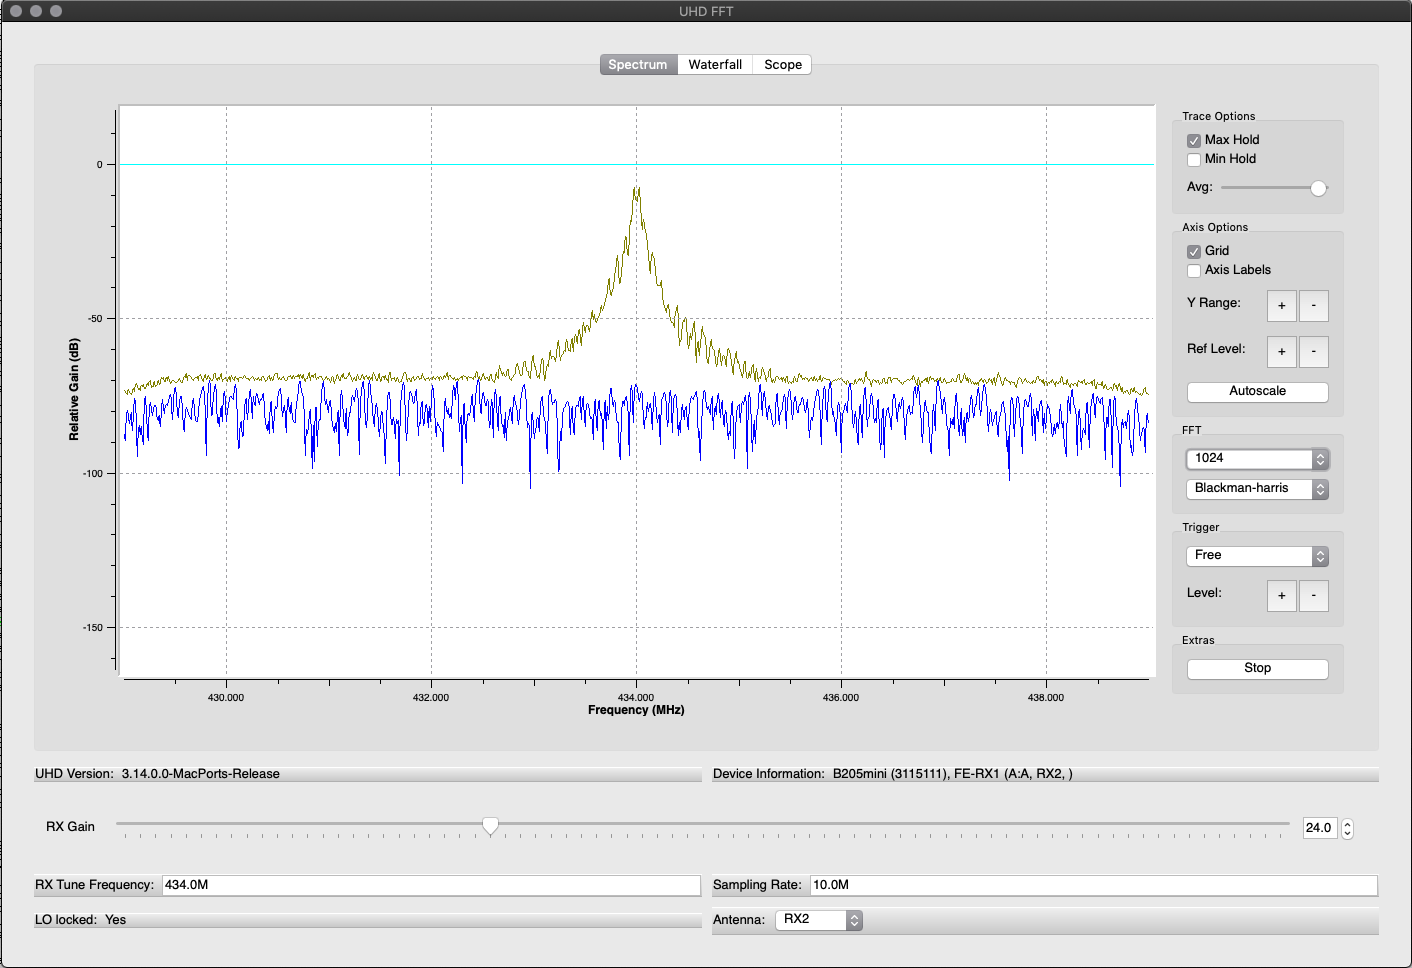
\includegraphics[width=\textwidth]{uhd_fft.png}
\caption{The output of the uhd\_fft command with a 434MHz signal present.}
\label{uhd_fft}
\centrefigureend

The spike on the yellow line in \cref{uhd_fft} shows that there is some signal present at the 434MHz frequency. We can change the settings on this window to see other signals which might be present, but first you need to run the following command from the command line to open the window.
\begin{lstlisting}
uhd_fft -f 434000000 -s 10000000
\end{lstlisting}
Try looking somewhere around 2.4GHz and seeing how busy it is. What do you think these signal might be?

\subsection{gnuradio flows}
Rather than using a prepackaged command like uht\_fft we can make our own \gls{gui}s using gnuradio companion. This can be a bit weird, so to start you off one has been provided. From the command line enter:
\begin{lstlisting}
gnuradio-companion 
\end{lstlisting}
From here open up the provided file FFT.grc and you can click the play button highlighted in \cref{grc_fft} and see the spectrum as we did before. At this point it's worth taking some time to familiarise yourself with gnuradio using the tutorial available here: \url{https://wiki.gnuradio.org/index.php/Guided\_Tutorial\_GRC}, that way it wont be a shock if the instruction is to 'add in the Throttle block', for example.

\centrefigurestart
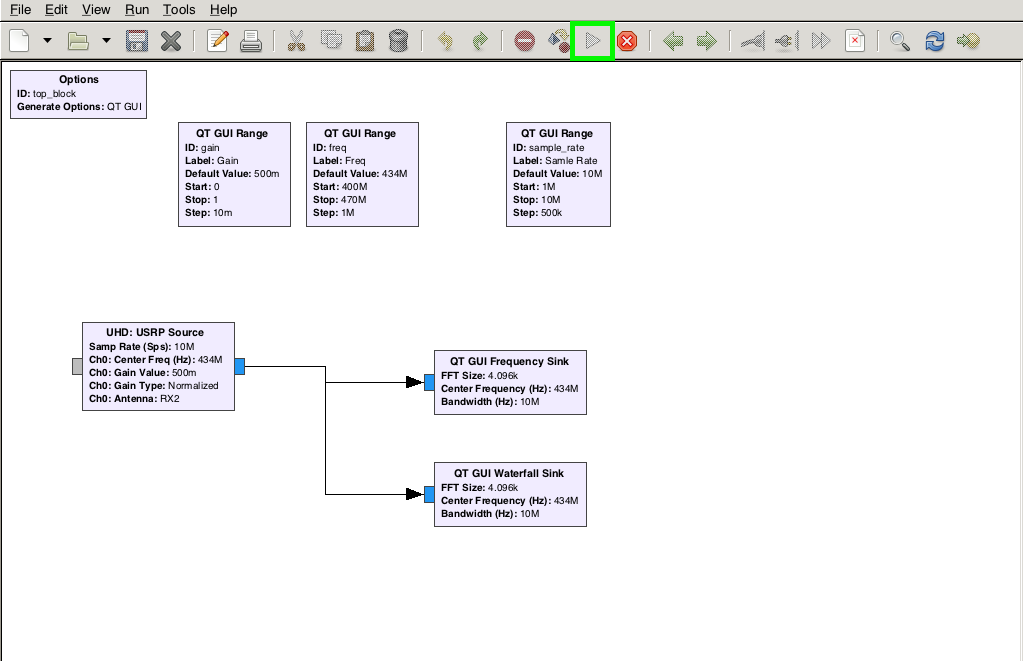
\includegraphics[width=\textwidth]{grc_fft.png}
\caption{gnuradio flow for viewing the spectrum}
\label{grc_fft}
\centrefigureend